%%%%%%%%%%%%%%%%%%%%%%%%%%%%%%%%%%%%%%%%%%%%%%%%%%%%%%%%%%%%%%%%%%%%%%%%%%%%%%%%%%
\begin{frame}[fragile]\frametitle{}
\begin{center}
{\Large Applications of Generative AI in Journalism}
\end{center}
\end{frame}

%%%%%%%%%%%%%%%%%%%%%%%%%%%%%%%%%%%%%%%%%%%%%%%%%%%%%%%%%%%%%%%%%%%%%%%%%%%%%%%%%%
\begin{frame}[fragile]\frametitle{Introduction to AI in Journalism}

\begin{itemize}
\item AI encompasses a range of technologies that simulate human intelligence.
\item Current capabilities include natural language processing (NLP), image recognition, and content generation.
\item These capabilities are transforming journalism by automating tasks and enhancing efficiency.
\item AI algorithms can analyze vast amounts of data quickly, leading to insights and story leads.
\item Journalists are increasingly relying on AI tools to streamline their workflow and produce high-quality content.
\end{itemize}

\end{frame}

%%%%%%%%%%%%%%%%%%%%%%%%%%%%%%%%%%%%%%%%%%%%%%%%%%%%%%%%%%%%%%%%%%%%%%%%%%%%%%%%%%
\begin{frame}[fragile]\frametitle{AI Applications in Journalism}

\begin{itemize}
\item Automated News Writing:  From structured data, such as financial reports or sports scores. Also in producing routine news stories quickly, freeing up journalists for more in-depth reporting.
\item Content Personalization (electronic media): based on individual preferences and interests.
\item Fact-Checking: Cross-referencing multiple sources and databases.
\item Audience Analytics: insights into audience preferences, helping journalists create content that resonates with their readers/viewers.
\end{itemize}

\end{frame}

%%%%%%%%%%%%%%%%%%%%%%%%%%%%%%%%%%%%%%%%%%%%%%%%%%%%%%%%%%%%%%%%%%%%%%%%%%%%%%%%%%
\begin{frame}[fragile]\frametitle{Advantages of AI in Journalism}

\begin{itemize}
\item Faster and More Efficient News Production: automates routine tasks like news writing, enabling journalists to focus on more complex stories.
\item Ability to Analyze and Process Large Volumes of Data: to uncover patterns and insights that may be overlooked by human journalists.
\item Personalized Content Delivery Based on User Preferences: delivering relevant stories and updates, increasing audience satisfaction and loyalty.
\end{itemize}

\end{frame}

%%%%%%%%%%%%%%%%%%%%%%%%%%%%%%%%%%%%%%%%%%%%%%%%%%%%%%%%%%%%%%%%%%%%%%%%%%%%%%%%%%
\begin{frame}[fragile]\frametitle{Challenges and Concerns}

\begin{itemize}
\item Potential Job Displacement and Automation of Journalistic Tasks: Journalists may need to acquire new skills to adapt to the changing landscape and work alongside AI systems.
\item Bias and Ethical Concerns in AI-Generated Content:
    \begin{itemize}
        \item May inadvertently perpetuate biases present in training data, leading to skewed or unfair news coverage.
        \item Ensuring fairness and impartiality in AI-generated content requires ongoing oversight and transparency.
    \end{itemize}
\item Credibility and Trust Issues with AI-Written Articles:
    \begin{itemize}
        \item Readers may question the credibility of news articles generated by AI, raising concerns about transparency and authenticity.
        \item Media organizations need to disclose the use of AI in content creation and uphold editorial standards to maintain trust with their audience.
    \end{itemize}
\item Privacy and Data Protection Concerns: Who OWNs the content, even though it is publicly available? Who is making money out of it? Who will take up legal cases for misinformation or defamation?
\end{itemize}

\end{frame}

%%%%%%%%%%%%%%%%%%%%%%%%%%%%%%%%%%%%%%%%%%%%%%%%%%%%%%%%%%%%%%%%%%%%%%%%%%%%%%%%%%
\begin{frame}[fragile]\frametitle{Case Studies and Examples}

\begin{itemize}
\item \textbf{The Washington Post's Heliograf}: to produce automated news stories on topics like sports, elections, and weather, allowing journalists to focus on more complex reporting.
\item \textbf{Reuters' Lynx Insights}: to analyze large datasets and identify news trends, to discover story leads and produce data-driven content across various beats.
\item \textbf{The Associated Press' AP Insights}: to personalize news content for its subscribers.
\item \textbf{BBC's Project Juicer}: to analyze audience engagement and optimize content distribution.
\end{itemize}

\end{frame}


%%%%%%%%%%%%%%%%%%%%%%%%%%%%%%%%%%%%%%%%%%%%%%%%%%%%%%%%%%%%%%%%%%%%%%%%%%%%%%%%%%
\begin{frame}[fragile]\frametitle{The Role of Human Journalists}

\begin{itemize}
\item Importance of Human Oversight, Editing, and Fact-Checking:to provide oversight and quality control, verifying information, detecting biases, and correcting errors in AI-generated content.
\item Unique Skills and Qualities that Human Journalists Bring:
    \begin{itemize}
        \item Critical thinking, intuition, and empathy, enabling them to contextualize news events and interpret complex issues for their audience.
        \item Storytelling prowess, investigative skills, and subject matter expertise that AI algorithms cannot replicate.
    \end{itemize}
\item Collaboration Between AI and Human Journalists: Complementary by automating routine tasks, analyzing data, and uncovering insights, allowing journalists to focus on higher-order tasks. Human with AI skills is more denagrious than just AI.
\end{itemize}

\end{frame}


%%%%%%%%%%%%%%%%%%%%%%%%%%%%%%%%%%%%%%%%%%%%%%%%%%%%%%%%%%%%%%%%%%%%%%%%%%%%%%%%%%
\begin{frame}[fragile]\frametitle{Ethical Considerations and Guidelines}

\begin{itemize}
\item Transparency and Disclosure: the use of AI in content creation and clearly label AI-generated content as such.
\item Fairness and Bias Mitigation:
    \begin{itemize}
        \item Journalists must be vigilant in identifying and addressing biases in AI algorithms and datasets to ensure fair and balanced news coverage.
        \item Regular audits and diversity assessments can help mitigate bias and promote inclusivity in AI-driven journalism.
    \end{itemize}
\item Accountability: Moral, Social, Legal (and Financial)
\item Privacy and Data Protection: Obtaining informed consent from users and adhering to data protection regulations help mitigate privacy risks and safeguard user information.
\end{itemize}

\end{frame}

%%%%%%%%%%%%%%%%%%%%%%%%%%%%%%%%%%%%%%%%%%%%%%%%%%%%%%%%%%%%%%%%%%%%%%%%%%%%%%%%%%
\begin{frame}[fragile]\frametitle{Future Trends and Predictions}

\begin{itemize}
\item Advancements in Natural Language Generation and Multimodal AI: capable of processing text, images, and audio together, will enable new forms of multimedia storytelling and news delivery.
\item Potential for AI to Enhance Investigative Journalism and Data-Driven Reporting: to conduct deeper investigations and analyze large datasets more efficiently.
\item Impact of AI on Media Business Models and Revenue Streams: to monetize content through subscription models and targeted advertising and will reduce operational costs and improve scalability, reshaping traditional media business models.
\end{itemize}

\end{frame}

%%%%%%%%%%%%%%%%%%%%%%%%%%%%%%%%%%%%%%%%%%%%%%%%%%%%%%%%%%%%%%%%%%%%%%%%%%%%%%%%%%
\begin{frame}[fragile]\frametitle{Strategies for Adaptation and Upskilling}

\begin{itemize}
\item Embrace Lifelong Learning: 
    \begin{itemize}
        \item You are domain (Journalism) expert. Need to know latest AI for usage in your domain. The Combination is Lethal, your niche.
        \item Participating in workshops, online courses, and professional development programs can help journalists acquire new skills and knowledge.
    \end{itemize}
\item Develop Data Literacy and Analytical Skills: Training in data analysis, statistics, and data visualization will enable journalists to interpret and communicate insights from large datasets.
\item Foster Collaboration and Interdisciplinary Teams: between journalists, data scientists, and AI experts to leverage diverse skills and perspectives.
\item Cultivate Ethical Awareness and Critical Thinking: Training in media ethics, bias detection, and algorithmic transparency will help journalists navigate ethical dilemmas in the AI-driven future.
\end{itemize}

\end{frame}

%%%%%%%%%%%%%%%%%%%%%%%%%%%%%%%%%%%%%%%%%%%%%%%%%%%%%%%%%%%%%%%%%%%%%%%%%%%%%%%%%%
\begin{frame}[fragile]\frametitle{Conclusion}

Opportunities

\begin{columns}
    \begin{column}[T]{0.6\linewidth}
		\begin{center}
		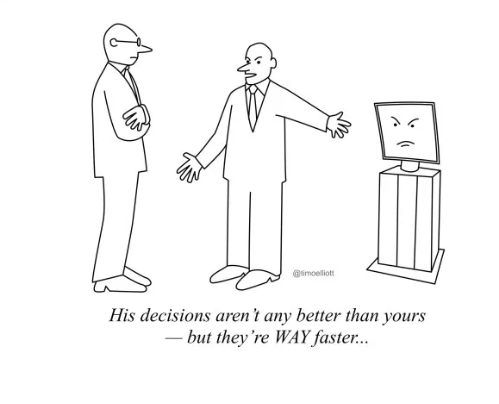
\includegraphics[width=\linewidth,keepaspectratio]{journalism1}
		
		{\tiny (ref: ProlitusTechnologies)}
		\end{center}

    \end{column}
    \begin{column}[T]{0.4\linewidth}

			\begin{itemize}
				\item To streamline workflows, analyze data, and engage audiences in innovative ways.
				\item Automated content generation, personalized news delivery, and data-driven reporting 
			\end{itemize}
    \end{column}
  \end{columns}
\end{frame}



%%%%%%%%%%%%%%%%%%%%%%%%%%%%%%%%%%%%%%%%%%%%%%%%%%%%%%%%%%%%%%%%%%%%%%%%%%%%%%%%%%
\begin{frame}[fragile]\frametitle{Conclusion}
Challenges
\begin{columns}
    \begin{column}[T]{0.6\linewidth}
		\begin{center}
		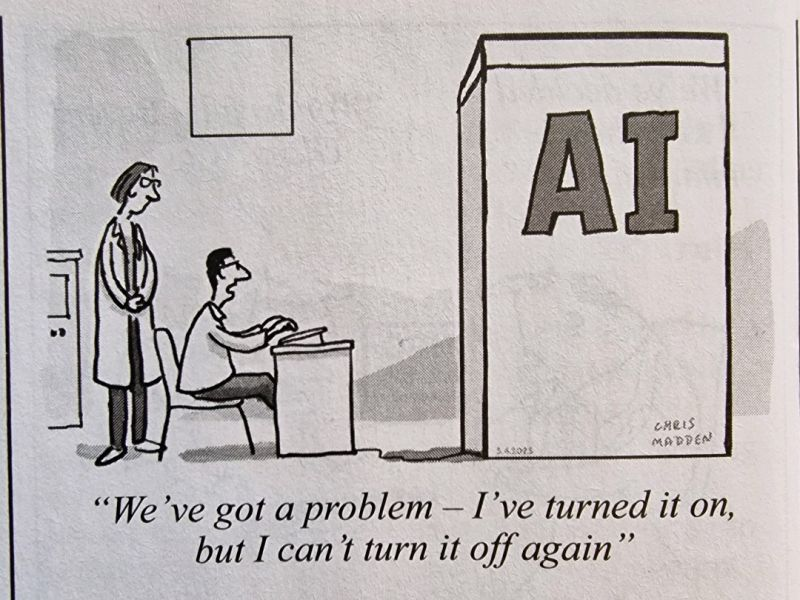
\includegraphics[width=\linewidth,keepaspectratio]{journalism2}
		
		{\tiny (ref: Ian McVicar on LinkedIn)}		
		\end{center}

    \end{column}
    \begin{column}[T]{0.4\linewidth}

			\begin{itemize}
				\item Ethical considerations, bias detection, and maintaining editorial standards
				\item Concerns about job displacement, privacy violations, and algorithmic accountability
			\end{itemize}
    \end{column}
  \end{columns}
\end{frame}


%%%%%%%%%%%%%%%%%%%%%%%%%%%%%%%%%%%%%%%%%%%%%%%%%%%%%%%%%%%%%%%%%%%%%%%%%%%%%%%%%%
\begin{frame}[fragile]\frametitle{Lessons Learnt}

\begin{itemize}
\item Embrace Lifelong Learning, Journalism + AI is the combination
\item Human Supervision cannot be removed from the journalistic process, so no full automation
\item AI models are as good as their training (data). Indic languages? non quantifiable data?
\item Human generated content will be more premium (but has to be better than ChatGPT)
\end{itemize}

\end{frame}